\documentclass[tikz, border=12pt]{standalone}
\usepackage{tikz}
\usepackage{xcolor}
\usepackage{amssymb}
\usetikzlibrary{shapes.geometric, arrows.meta, positioning, fit, backgrounds, shadows, calc}

% ── Colours ──────────────────────────────────────────────────────────────────
\definecolor{colHal}    {RGB}{ 30,  90, 160}   % HAL source  – deep blue
\definecolor{colAsm}    {RGB}{  0, 140, 180}   % Assembler   – cyan-blue
\definecolor{colHlx}    {RGB}{ 30, 150,  80}   % .hlx output – green
\definecolor{colCrun}   {RGB}{180,  80,  30}   % crun        – orange
\definecolor{colOut}    {RGB}{140,  30, 140}   % output      – purple
\definecolor{colSide}   {RGB}{ 90, 100, 115}   % side files  – steel
\definecolor{colPanel}  {RGB}{240, 244, 250}   % panel bg
\definecolor{colDark}   {RGB}{ 40,  50,  65}   % dark text

% ── Styles ───────────────────────────────────────────────────────────────────
\tikzset{
  filenode/.style 2 args={
    rectangle, rounded corners=7pt,
    draw=#1!75!black, fill=#1!18, text=colDark,
    font=\sffamily\bfseries\small,
    minimum width=2.6cm, minimum height=1.1cm,
    drop shadow={shadow xshift=2pt, shadow yshift=-2pt, opacity=0.25},
    align=center, inner sep=6pt
  },
  procnode/.style 2 args={
    rectangle, rounded corners=5pt,
    draw=#1!85!black, fill=#1, text=white,
    font=\sffamily\bfseries\normalsize,
    minimum width=3.8cm, minimum height=1.3cm,
    drop shadow={shadow xshift=2pt, shadow yshift=-2pt, opacity=0.30},
    align=center, inner sep=8pt
  },
  sidenode/.style={
    rectangle, rounded corners=5pt,
    draw=colSide!60, fill=colSide!10, text=colDark,
    font=\sffamily\footnotesize,
    minimum width=2.2cm, minimum height=0.85cm,
    align=center, inner sep=5pt
  },
  fatarrow/.style={
    -Stealth, line width=2.2pt, color=#1,
    shorten >=2pt, shorten <=2pt
  },
  thindasharrow/.style={
    -Stealth, dashed, line width=1pt, color=colSide,
    shorten >=2pt, shorten <=2pt
  },
  lbl/.style={
    font=\sffamily\tiny\itshape, text=colSide,
    fill=white, inner sep=2pt
  },
  sublbl/.style={
    font=\sffamily\scriptsize, text=white!85,
    align=center
  },
}

\begin{document}
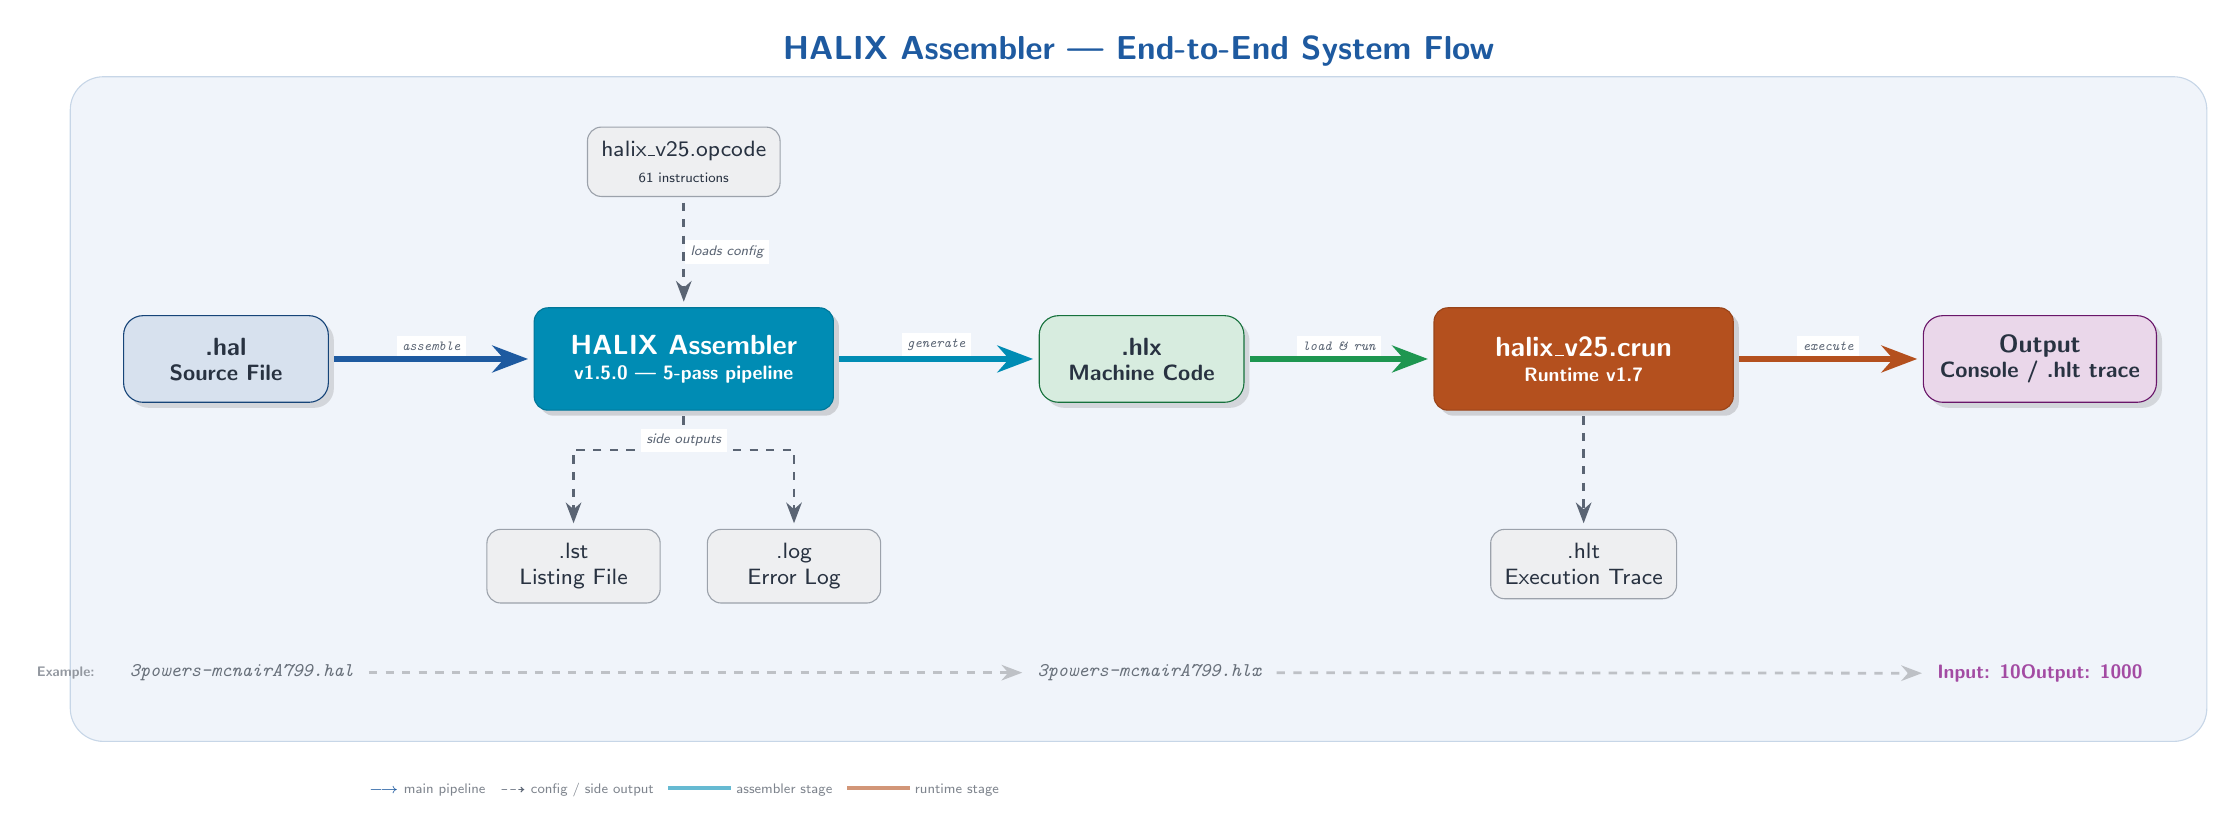
\begin{tikzpicture}[node distance=1.6cm and 2.4cm]

%% ══════════════════════════════════════════════════════════════
%%  MAIN PIPELINE  (left → right, horizontal)
%% ══════════════════════════════════════════════════════════════

% 1. HAL source file
\node[filenode={colHal}{}] (hal) {.hal\\[-2pt]{\footnotesize Source File}};

% 2. HALIX Assembler box
\node[procnode={colAsm}{}, right=2.6cm of hal] (asm)
  {HALIX Assembler\\[-3pt]\scriptsize v1.5.0 — 5-pass pipeline};

% 3. .hlx machine code
\node[filenode={colHlx}{}, right=2.6cm of asm] (hlx)
  {.hlx\\[-2pt]{\footnotesize Machine Code}};

% 4. crun runtime
\node[procnode={colCrun}{}, right=2.4cm of hlx] (crun)
  {halix\_v25.crun\\[-3pt]\scriptsize Runtime v1.7};

% 5. Program output
\node[filenode={colOut}{}, right=2.4cm of crun] (out)
  {Output\\[-2pt]{\footnotesize Console / .hlt trace}};

%% ── main arrows ─────────────────────────────────────────────
\draw[fatarrow=colHal] (hal)  -- node[lbl,above]{\texttt{assemble}} (asm);
\draw[fatarrow=colAsm] (asm)  -- node[lbl,above]{\texttt{generate}} (hlx);
\draw[fatarrow=colHlx] (hlx)  -- node[lbl,above]{\texttt{load \& run}} (crun);
\draw[fatarrow=colCrun](crun) -- node[lbl,above]{\texttt{execute}} (out);

%% ══════════════════════════════════════════════════════════════
%%  SIDE OUTPUTS of assembler  (below asm)
%% ══════════════════════════════════════════════════════════════
\node[sidenode, below=1.5cm of asm, xshift=-1.4cm] (lst) {.lst\\Listing File};
\node[sidenode, below=1.5cm of asm, xshift= 1.4cm] (log) {.log\\Error Log};

\draw[thindasharrow] (asm.south) -- ++(0,-0.5) -| (lst.north);
\draw[thindasharrow] (asm.south) -- ++(0,-0.5) -| (log.north);

\node[lbl, below=0.22cm of asm] {side outputs};

%% ══════════════════════════════════════════════════════════════
%%  CONFIG INPUT  (above asm)
%% ══════════════════════════════════════════════════════════════
\node[sidenode, above=1.4cm of asm] (opcode)
  {halix\_v25.opcode\\{\tiny 61 instructions}};
\draw[thindasharrow] (opcode.south) -- node[lbl,right]{loads config} (asm.north);

%% ══════════════════════════════════════════════════════════════
%%  EXECUTION TRACE output of crun  (below crun)
%% ══════════════════════════════════════════════════════════════
\node[sidenode, below=1.5cm of crun] (hlt) {.hlt\\Execution Trace};
\draw[thindasharrow] (crun.south) -- (hlt.north);

%% ══════════════════════════════════════════════════════════════
%%  EXAMPLE ROW  (below main pipeline, shows real values)
%% ══════════════════════════════════════════════════════════════
\node[font=\sffamily\scriptsize\itshape, text=colDark!70,
      below=3.2cm of hal, xshift=0.2cm]
  (ex1) {\texttt{3powers-mcnairA799.hal}};

\node[font=\sffamily\scriptsize\itshape, text=colDark!70,
      below=3.2cm of hlx, xshift=0.1cm]
  (ex2) {\texttt{3powers-mcnairA799.hlx}};

\node[font=\sffamily\scriptsize\bfseries, text=colOut!80,
      below=3.2cm of out]
  (ex3) {Input: 10\\Output: \textbf{1000}};

% dashed connectors for example row
\draw[thindasharrow, color=colDark!30] (ex1.east) -- (ex2.west);
\draw[thindasharrow, color=colDark!30] (ex2.east) -- (ex3.west);

\node[font=\sffamily\tiny\bfseries, text=colDark!50,
      left=0.2cm of ex1] {Example:};

%% ══════════════════════════════════════════════════════════════
%%  BACKGROUND PANELS
%% ══════════════════════════════════════════════════════════════
\begin{scope}[on background layer]
  % assembler sub-panel
  \node[fill=colAsm!8, draw=colAsm!30, rounded corners=8pt,
        fit=(asm)(opcode)(lst)(log),
        inner sep=10pt] {};

  % crun sub-panel
  \node[fill=colCrun!8, draw=colCrun!30, rounded corners=8pt,
        fit=(crun)(hlt), inner sep=10pt] {};

  % outer panel
  \node[fill=colPanel, draw=colHal!25, rounded corners=12pt,
        fit=(hal)(asm)(hlx)(crun)(out)(opcode)(lst)(log)(hlt)(ex1)(ex2)(ex3),
        inner sep=18pt,
        label={[font=\sffamily\bfseries\large, text=colHal]
               above:HALIX Assembler — End-to-End System Flow}] {};
\end{scope}

%% ══════════════════════════════════════════════════════════════
%%  LEGEND
%% ══════════════════════════════════════════════════════════════
\node[font=\sffamily\tiny, text=colDark!60,
      below=4.6cm of asm]
  {\textcolor{colHal}{$\longrightarrow$}\ main pipeline\quad
   \textcolor{colSide}{$\dashrightarrow$}\ config / side output\quad
   \textcolor{colAsm!60}{\rule[0.5ex]{0.8cm}{1.5pt}}\ assembler stage\quad
   \textcolor{colCrun!60}{\rule[0.5ex]{0.8cm}{1.5pt}}\ runtime stage};

\end{tikzpicture}
\end{document}
